\documentclass{article}

%packeges
\usepackage{bytefield} %Protokoldarstellung
\usepackage{vhistory} %Dokmentationshistorie
\usepackage[german]{babel} %deutsche Sprache
\usepackage[utf8]{inputenc}
\usepackage[
	colorlinks=true,
	urlcolor=blue,
	linkcolor=black
]{hyperref} %Links zu Libraries

%create title
\title{Project Contemplant - Arduino}
\date{Juni 19, 2018}
\author{Montag 1}

\begin{document}
\maketitle
% Versionshistorie
\begin{versionhistory}
  \vhEntry{0.1}{19.06.2018}{Marcus Leibner}{Initiale Version}
\end{versionhistory}
\newpage

\tableofcontents
\newpage
\section{Allgemeines}
Der Arduino dient zur Erfassung und Weiterleitung einiger Umweltdaten, welche zur Evaluierung eines Lernraumes benötigt werden, dies geschieht sobald der Nutzer seine personalisierte Pflanze über das Webinterface auf den Arduino geladen hat. \newline
Des Weiteren stellt er die aktuellen Daten auf einem Bildschrim dar, damit der User während seiner Lernzeit immer über den Raum informiert bleibt, ohne auf sein Handy o.Ä. zu schauen.
\newpage

\section{Kommunikation}
%sollte Allgemeine Funktionsweise + Infos über die Kommunikation enthalten
\subsection{Allgemeines}
Dieser Abschnitt befasst sich mit der Kummunikation zwischen dem Arduino und dem Raspberry PI.\newline
Bei der Kommunikation herrscht eine 1 zu n Beziehung es gibt einen Raspberry PI, welcher mit n Arduinos kommunizieren kann, 
hierzu werden XBee-Module genutzt (Funkverbindung).\newline
%war mir im Code jetzt nicht ersichtlich, ich habe das erstmal hingeschrieben, weil ich der Meinung war, das sollte das Interval sein
Das Zeitintervall in dem die Daten geschickt werden beträgt 10 Sekunden.\newline
%genaue Spezifikation und Erläuterung des Protokols
\subsection{Protokol}
Das Protokoll ist 24 Byte groß und besteht aus folgenden Daten: \newline
Flags: ? \newline
sourceID: Dient zur Identifizierung des sendenden Arduinos und beeinhaltet die Arduino ID.\newline
Compression: ? \newline
Timestamp: Der Zeitstempel wird in der Unixzeit geschickt (vergangene Sekunden seit 1970.01.01) 
und dient dazu die Daten differenzieren zu können.\newline
Temperature: Enthält die ermittelte Temperatur.\newline
Humidity: Enthält die ermittelte Feuchtigkeit (in diesem Fall Luftfeuchtigkeit).\newline
Radiation: Enthält die ermittelte Sonneneinstrahlung.\newline
Loudness: Enthält diue ermittelte Lautstärke.\newline
\newline
\begin{bytefield}[bitwidth=1.1em]{32}
\bitheader{0-31} \\
\bitbox{8}{Flags} & \bitbox{16}{sourceID} & \bitbox{8}{Compression} \\
& \bitbox{32}{Timestamp} \\
& \bitbox{32}{Temperature}\\
& \bitbox{32}{Humidity} \\
& \bitbox{32}{Radiation} \\
\bitbox{32}{Loudness}
\end{bytefield}
\subsection{XBee}
%eventuell Screenshots der Konfiguaration + Erläuterung
TODO\newline
\newpage

%Erläuterung zu genutzten Sensoren und Aktoren
\section{Sensoren und Aktoren}
%Aufzählung aller Sensoren + Beschreibung (falls jemand das genaue Produkt finden sollte, kann er es gerne mit reinhauen)
\subsection{Sensoren}
Zur Erfassung der Umweltdaten werden folgende Sensoren verwendet: \newline
Temperatursensor\textsuperscript{\ref{Temperature}}: 
Dient zur Erfassung der Außentemperatur.\newline
Feuchtigkeitssensor: 
Dient zur Erfassung der Luftfeuchtigkeit.\newline
Lichtsensor\textsuperscript{\ref{Light}}: 
Dient zur Erfassung der Lichteinstrahlung.\newline
Lautstärkesensor: 
Dient zur Erfassung der Lautstärke. \newline
Echtzeituhr\textsuperscript{\ref{RTC}}: 
Dient zur Ermittlung der aktuellen Zeit (Jahr-Monat-Tag-Stunden-Minuten-Sekunden), 
diese wird auf dem Arduino in die Unixzeit umgerechnet.\newline
Druckknopf: 
Führt bei Betätigung zum Entladen der derzeitig geladenen Pflanze.\newline
%Aufzählung aller Aktoren + Beschreibung
\subsection{Aktoren}
Der Arduino verwendet folgende Aktoren: \newline
Bildschirm\textsuperscript{\ref{LCD}}: 
Der Bildschirm hat eine Auflösung von (?/?) und dient zur Anzeige der aktuellen Umweltbedingungen.\newline
XBee\textsuperscript{\ref{Xbee}}: 
Dient zur Kommunikation mit dem Raspberry PI über eine Funkverbindung.
%Was passiert in Ausnahmefällen
\newpage

\section{Simulation}

\subsection{Die Umgebungsfunktion}

Gesucht wurde eine Funktion, die aus den eingelesenen Sensordaten einen Wert berechnet, der angibt wie gut die Umgebungsvariablen (Helligkeit, Temperatur, Luftfeuchtigkeit, Lautstärke) für die Pflanze sind.\\
Der User gibt für jede Umgebungsvariable seinen Optimalwert (der Wert bei dem er am besten Lernen kann, bspw. 20°C für die Temperatur) und die Gewichtung an, je nachdem wie stark die jeweilige Umgebungsvariable den berechneten Umgebungswert beeinflussen soll. Der Hintergedanke hierbei war, dass jeder User weiß, unter welchen Bedingungen er am besten lernen kann.\\
Die Abweichung der Umgebungsvariable von dem Optimalwert soll also den Umgebungswert negativ beeinflussen. Hierzu haben wir uns folgende Kriterien überlegt:\\
- Bei kleineren Abweichungen sollte der Umgebungswert erst nicht so schnell fallen.\\
- Es sollte eine maximale Abweichung geben, ab der der Wert stets 0 ist für die jeweilige Umgebungsvariable.\\
Die Funktion sieht wiefolgt aus, wobei auf der x-Achse die Abweichung vom Optimalwert dargestellt wird:\\

\begin{figure*}[h!]
\centering
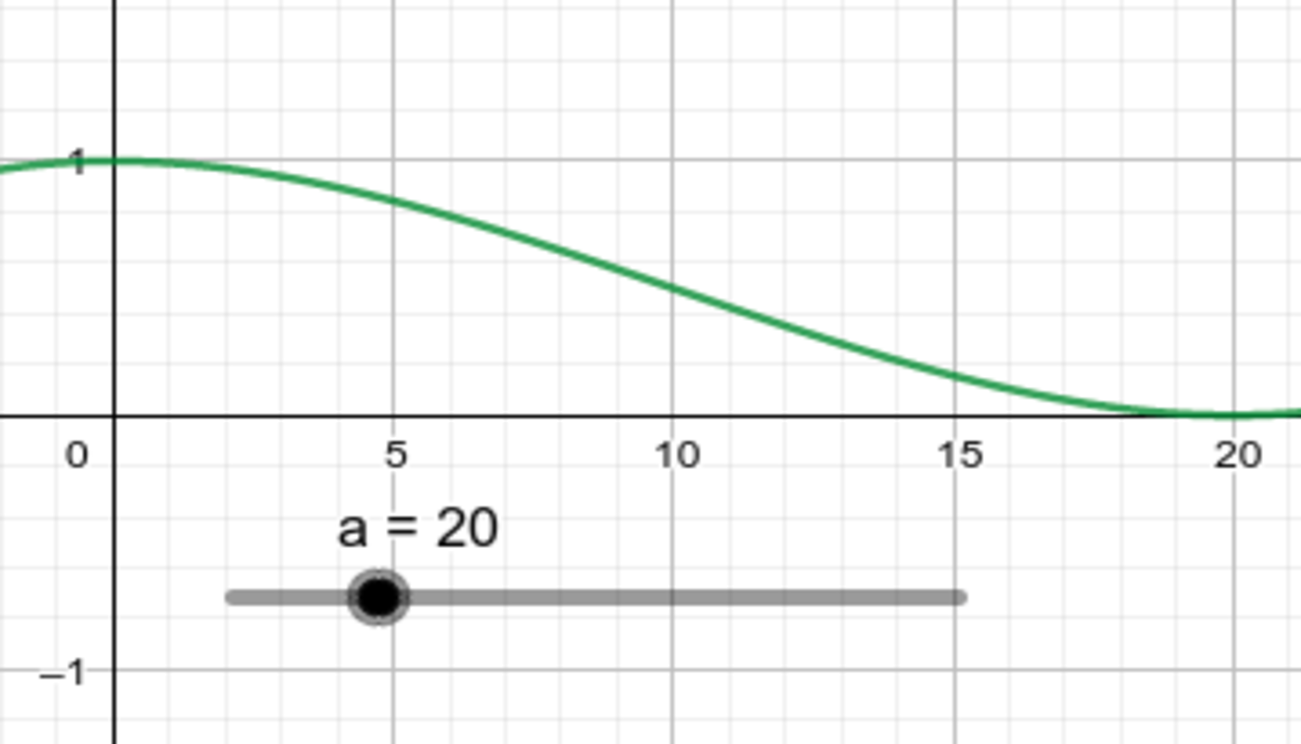
\includegraphics[width=0.5\textwidth]{fnct.png}
\caption{max = 20}
\end{figure*}

\begin{align*}
f(x) = 
\frac{2}{max^3} \cdot x^3 - \frac{3}{max^2}\cdot x^2 + 1
\end{align*}

Seien $f_i$ die Werte die die Umgebungsfunktion für den Sensor i ausgibt und seien $w_i$ die Gewichtung des jeweiligen Sensors. Dann berechnet man den Umgebungswert für n Sensoren folgendermaßen:

\begin{align*}
env(\boldsymbol{f},\boldsymbol{w}) = \sum_{i=0}^{n} (f_i \cdot w_i)
\end{align*}


\section{Errorhandling}
\subsection{Raspberry PI nicht erreichbar}
Wenn der Raspberry PI nicht erreichbar ist speichert der Arduino alle nicht-versendbaren Pakete und schickt diese, sobald wieder eine Verbindung besteht.\newline
%hier sollte noch eine Beschreibung der Komprimierung hin, also welche Daten gehen verloren, wie wird Kompromiert etc.
\subsection{Keine Stromzufuhr}
Wenn der Arduino vom Strom getrennt wird und nach einiger Zeit wieder an den Strom angebunden ist, ist der zuletzt angemeldete Nutzer weiterhin angemeldet und muss sich nicht nocheinmal neu anmelden.\newline
\newpage

\section{Libraries}
Folgende C-Libraries wurden zur Realisierung des Projekts auf dem Arduino verwendet: \newline
%rove Digital Light Sensor\footnote{\label{Light}\url{http://wiki.seeedstudio.com/Grove-Digital_Light_Sensor/}}\newline
Grove Sunlight Sensor\footnote{\label{Light}\url{http://wiki.seeedstudio.com/Grove-Sunlight_Sensor/}}\newline
Grove Temperature Sensor\footnote{\label{Temperature}\url{http://wiki.seeedstudio.com/Grove-Temperature_Sensor/}}\newline
I2C LCD Library\footnote{\label{LCD}\url{TODO}}\newline
RTC Library\footnote{\label{RTC}\url{http://wiki.seeedstudio.com/Grove-RTC/}}\newline
Xbee Arduino\footnote{\label{Xbee}\url{https://github.com/andrewrapp/xbee-arduino}}\newline

\end{document}